\documentclass[a4paper]{article}
\usepackage[T1]{fontenc}
\usepackage[english]{babel}
\usepackage{clrscode4e} % Algorithm template from Introduction to Algorithms 4th
\usepackage[left=2cm,right=2cm,top=1cm,bottom=2cm]{geometry} % page settings
\usepackage{amsthm, amsmath} % provides many mathematical environments & tools
\usepackage{tikz} % draw pictures
\usepackage{tabularray}
\usepackage[noend]{algorithmic}
\usepackage{tabularx}
\usepackage[noend]{algorithmic}
\usepackage{algorithm}
\usepackage{arydshln}
\usepackage{forest}
\usepackage{adjustbox}
\usepackage{array}
\usepackage{ifthen}
\usepackage{caption}
\usepackage{subfig}
\usepackage{graphicx,wrapfig,lipsum}
%-----------------------------------------------------------
% Custom commands
%-----------------------------------------------------------
\newenvironment{hashtable}[1][]
  {\begin{tabular}[#1]{
     @{}
     > {\small} r <{\normalsize~\rlap{\fbox{\strut~~}}$~~\rightarrow$~}
     @{} l @{}}}
  {\end{tabular}}

\tikzset{
node of list/.style = {
             draw,
             fill=orange!20,
             minimum height=6mm,
             minimum width=6mm,
             node distance=6mm
   },
link/.style = {
     -stealth,
     shorten >=1pt
     },
array element/.style = {
    draw, fill=white,
    minimum width = 6mm,
    minimum height = 10mm
  }
}

\def\LinkedList#1{%
  \foreach \element in \list {
     \node[node of list, right = of aux, name=ele] {\element};
     \draw[link] (aux) -- (ele);
     \coordinate (aux) at (ele.east);
  }
}

\usetikzlibrary{positioning,matrix, arrows.meta}
\tikzset{box/.style={draw, thick, minimum width=1cm, minimum height=1cm}}

\newenvironment{solution}
  {\begin{proof}[Solution]}
  {\end{proof}}
\renewcommand{\qedsymbol}{\rule{0.7em}{0.7em}}

\makeatletter
\renewenvironment{proof}[1][\proofname]{%
  \par\pushQED{\qed}\normalfont%
  \topsep6\p@\@plus6\p@\relax
  \trivlist\item[\hskip\labelsep\bfseries#1\@addpunct{.}]%
  \ignorespaces
}{%
  \popQED\endtrivlist\@endpefalse
}
\makeatother

\tikzset{
      heap/.style={
        every node/.style={circle,draw,minimum width=8mm},
        level 1/.style={sibling distance=80mm},
        level 2/.style={sibling distance=50mm},
        level 3/.style={sibling distance=20mm}, % <----- Here's the lowest level of your tree
        level 4/.style={sibling distance=10mm}
      }
    }

\setlength{\parindent}{0mm}

%-----------------------------------------------------------
% Document
%-----------------------------------------------------------
\begin{document}

\title{Algorithms: Homework 2}
\author{Li-Yuan Wei}
\date{\today}
\maketitle

\subsection*{Problem 1}
\begin{solution}
\end{solution}

\subsection*{Problem 2}
\begin{solution}
  ??
\end{solution}

\subsection*{Problem 3}
\begin{figure}[H]
\centering
\begin{minipage}{5cm}
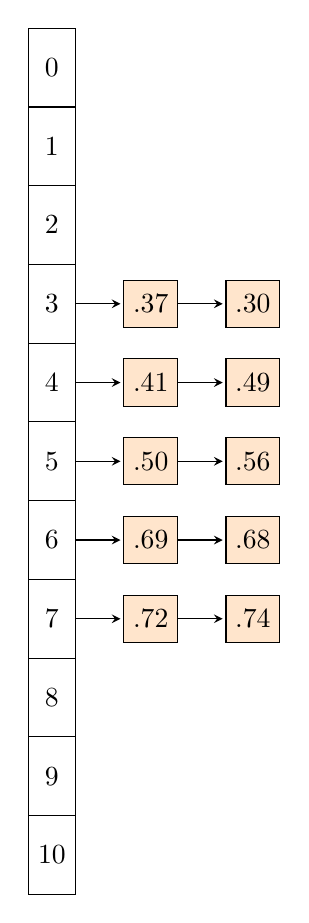
\begin{tikzpicture}
  \foreach \index/\list in {0/{}, 1/{}, 2/{}, 3/{.37,.30}, 4/{.41, .49}, 5/{.50, .56}, 6/{.69, .68}, 7/{.72, .74}, 8/{}, 9/{}, 10/{}} {
   \node[array element] (aux) at (0,-\index) {\index};
   \LinkedList{\list}
}
\end{tikzpicture}
\caption{Insert data}
\end{minipage}
\qquad
\begin{minipage}{5cm}
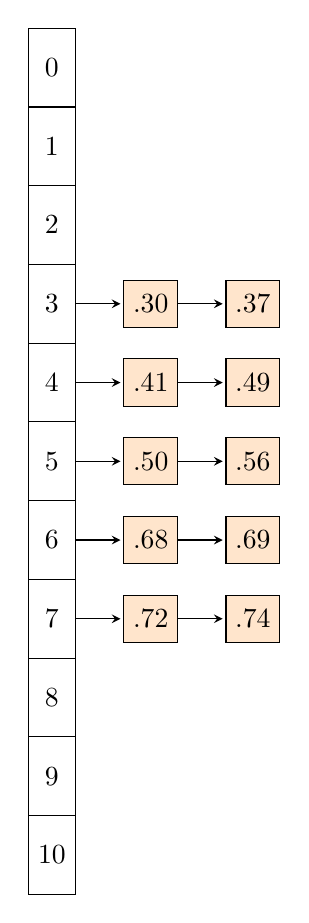
\begin{tikzpicture}
  \foreach \index/\list in {0/{}, 1/{}, 2/{}, 3/{.30,.37}, 4/{.41, .49}, 5/{.50, .56}, 6/{.68, .69}, 7/{.72, .74}, 8/{}, 9/{}, 10/{}} {
   \node[array element] (aux) at (0,-\index) {\index};
   \LinkedList{\list}
}
\end{tikzpicture}
\caption{Sort each bucket}
\end{minipage}
\end{figure}

\subsection*{Problem 4}
\begin{solution}
\end{solution}

\subsection*{Problem 5}
\begin{solution}

\end{solution}

\subsection*{Problem 6}
\begin{figure}[H]
\centering
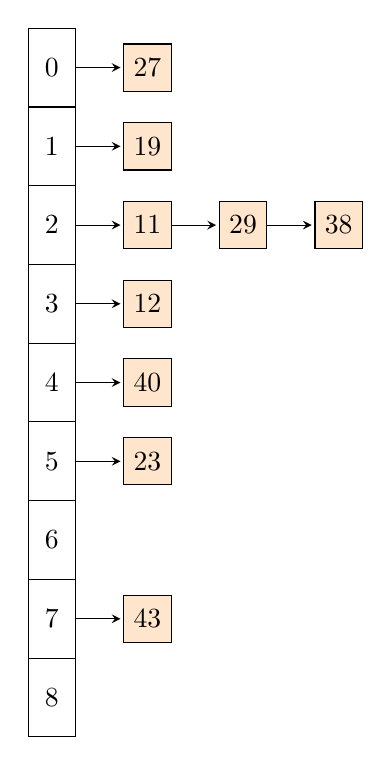
\begin{tikzpicture}
  \foreach \index/\list in {0/{27}, 1/{19}, 2/{11,29,38}, 3/{12}, 4/{40}, 5/{23}, 6/{}, 7/{43}, 8/{}} {
   \node[array element] (aux) at (0,-\index) {\index};
   \LinkedList{\list}
}
\end{tikzpicture}
\caption{Hash table with chaining}
\end{figure}

\subsection*{Problem 7}
\begin{figure}[H]
\centering
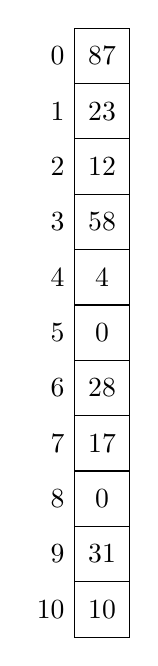
\begin{tikzpicture}
\coordinate (0);
\foreach \t[count=\i from 0,evaluate=\i as\j using int(\i+1)] in {
  87,
  23,
  12,
  58,
  4,
  0,
  28,
  17,
  0,
  31,
  10
}
\node at(\i.south)[anchor=north,draw,minimum height=2em,minimum width=2em,outer sep=0pt](\j){\t}
    node at(\j.west)[align=right,left]{\i}
    node at(\j.east)[align=left,right,xshift=-.7em]{};
\end{tikzpicture}
\caption{linear probing}
\end{figure}

\begin{figure}[H]
\centering
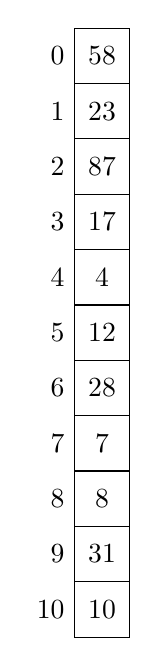
\begin{tikzpicture}
\coordinate (0);
\foreach \t[count=\i from 0,evaluate=\i as\j using int(\i+1)] in {
  58,
  23,
  87,
  17,
  4,
  12,
  28,
  7,
  8,
  31,
  10
}
\node at(\i.south)[anchor=north,draw,minimum height=2em,minimum width=2em,outer sep=0pt](\j){\t}
    node at(\j.west)[align=right,left]{\i}
    node at(\j.east)[align=left,right,xshift=-.7em]{};
\end{tikzpicture}
\caption{quadratic probing}
\end{figure}

\begin{figure}[H]
\centering
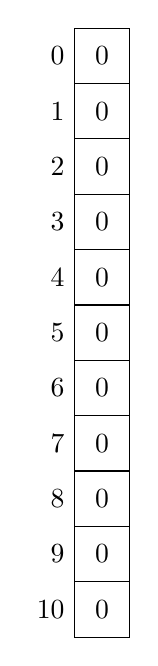
\begin{tikzpicture}
\coordinate (0);
\foreach \t[count=\i from 0,evaluate=\i as\j using int(\i+1)] in {
  0,
  0,
  0,
  0,
  0,
  0,
  0,
  0,
  0,
  0,
  0
}
\node at(\i.south)[anchor=north,draw,minimum height=2em,minimum width=2em,outer sep=0pt](\j){\t}
    node at(\j.west)[align=right,left]{\i}
    node at(\j.east)[align=left,right,xshift=-.7em]{};
\end{tikzpicture}
\caption{double hashing}
\end{figure}

\subsection*{Problem 8}
\begin{solution}
\end{solution}

\subsection*{Problem 9}
\begin{solution}
\end{solution}

\begin{figure}[H]
\centering
\parbox{5cm}{
\caption{First.}
\label{fig:2figsA}}
\qquad
\begin{minipage}{5cm}
\caption{Second.}
\label{fig:2figsB}
\end{minipage}
\begin{minipage}{5cm}
\caption{Third.}
\label{fig:3figsC}
\end{minipage}
\end{figure}

\subsection*{Problem 10}
\begin{solution}
\end{solution}

\begin{tblr}{|l|c|r|}
\hline
 Left & {Center \\ Cent \\ C} & {Right \\ R} \\
\hline
{L \\ Left} & {C \\ Cent \\ Center} & R \\
\hline
\end{tblr}

\end{document}


